\documentclass[journal]{IEEEtran}

\ifCLASSINFOpdf
   \usepackage[pdftex]{graphicx}
\else

\fi
%encoding
\usepackage{fancybox}
%--------------------------------------
\usepackage[utf8]{inputenc}
\usepackage[T1]{fontenc}
\usepackage{pgfplots}
\usepackage{subfig}
% Define o caminho das figuras

\usepackage{nomencl}
\usepackage{hyphenat}
\hyphenation{op-tical net-works semi-conduc-tor}

%--------------------------------------
 
%Portuguese-specific commands
%--------------------------------------
%\usepackage[portuguese]{babel}
\usepackage[english,american]{babel}
%--------------------------------------
 
%Hyphenation rules
%--------------------------------------
\usepackage{hyphenat}
\hyphenation{mate-mática recu-perar}
%--------------------------------------
\usepackage{graphicx}
\usepackage{placeins}
\usepackage{balance}
\usepackage{color,graphicx}

% correct bad hyphenation here
\hyphenation{op-tical net-works semi-conduc-tor}


\begin{document}
%
% paper title

\title{An Automated Testing Environment For The ITU-I/ISO-IEC Reference Video Encoders}
%

\author{José Raimundo Barbosa,~\IEEEmembership{~Instituto Federal da Paraíba - Campus João Pessoa};
        Jean Felipe Fonseca de Oliveira,~\IEEEmembership{Samsung, São Paulo, Brasil};
        Carlos Danilo Miranda Regis,~\IEEEmembership{~Instituto Federal da Paraíba - Campus João Pessoa}
        and~Ruan Delgado Gomes,~\IEEEmembership{~Instituto Federal da Paraíba - Campus Campina Grande}% <-this % stops a space
\thanks{M. Shell was with the Department
of Electrical and Computer Engineering, Georgia Institute of Technology, Atlanta,
GA, 30332 USA e-mail: (see http://www.michaelshell.org/contact.html).}% <-this % stops a space
\thanks{J. Doe and J. Doe are with Anonymous University.}% <-this % stops a space
\thanks{Manuscript received April 19, 2005; revised August 26, 2015.}}

% The paper headers
\markboth{JOURNAL OF COMMUNICATION AND INFORMATION SYSTEMS,~Vol.~33, No.~1, Definir~2018}%
{Shell \MakeLowercase{\textit{et al.}}: Bare Demo of IEEEtran.cls for IEEE Journals}

% make the title area
\maketitle

% As a general rule, do not put math, special symbols or citations
% in the abstract or keywords.
\begin{abstract}
The ITU-T/ISO-IEC H.265/HEVC is the state-of-the-art video codec, focusing in Ultra-High Definition video (UHD) and it is about two times more efficient in bit-rate compression than its predecessor, the H.264/AVC. However, this efficiency requires a high computational cost, which may compromise the use of the encoder in limited machines or in real time applications that use UHD videos. Several studies look for ways to enhance the HEVC encoder and reduce the computational cost. However, to develop optimized versions of the encoder it is necessary to perform tests that can last for hours and usually requires manual collection of coding information.  In this work, a tool to perform automated tests of HEVC encoders  was developed. The tool was implemented in a parallel architecture that allows the execution of several instances of the encoder simultaneous. It collects the informations from the encoders and executes objective metrics to evaluate its efficiency, organizes the results and generates reports. This work intends to provide an useful solution to help video coding researchers analyzing encoders in long sequences of tests.
\end{abstract}

% Note that keywords are not normally used for peerreview papers.
\begin{IEEEkeywords}
Automated Testing, Video Encoder.
\end{IEEEkeywords}


\IEEEpeerreviewmaketitle


\section{Introduction}

%JEAN: Tenta atualizar esse dado da cisco. Eles acabaram de lançar os dados para 2016-2021.
Currently, about three-quarters of annual data traffic on the Internet is assigned to video content, according to Cisco's Visual Networking Index report. 
%In 2014 this consumption was 64\% and\end{comment} 
In 2020 this value will be about 80\%~\cite{Cisco:16}. One of the contributing factors is the increasing in video quality, which enables new experiences on Internet-broadcast television channels, video conferencing and on-demand video transmission services such as YouTube, Amazon and Netflix, which already distribute UHD videos~\cite{cheon:14}.


The amount of pixels in UHD videos leads to an significant improvement in the perception of image details, allowing new experiences for viewers, but it also represents challenges to current market~\cite{cheon:14}. For example, a UHD 4K video has a resolution of 4096x2160 pixels, while previous standards such as Full HD have 1920x1080. Considering a raw uncompressed UHD 4K video sequence, with 24 bits per pixel and 24 frames per second, it would require a bandwidth of 5 Gbit/s~\cite{gomes:13}. These settings represent challenges in the storage and transmission of such videos.

In order to handle the intense and growing traffic of UHD videos over the Internet and to address the bandwidth limitations, it was necessary to develop new codecs of significantly reduce transmitted data volume without sacrifice the perceived visual quality~\cite{oliveira:16}\cite{wang:13}~\cite{netflix:16}. The ITU-T H.265~\cite{itu:265}, also known as High Efficiency Video Coding (HEVC), is the state-of-the-art codec which focus primarily on the newest UHD video technologies and presents a compression efficiency two times higher than its predecessor, the H.264/Advanced Video Coding (AVC)~\cite{Bossen:12}\cite{Hanhart:12}\cite{Sullivan:12}. To reach the aforementioned performance, the HEVC standard implements several enhancements in relation to the H.264, such as the Quadtree Partitioning Scheme and the increased number of intra predicition modes (HEVC has 33 modes while H.264 has 9). However, all these changes leads to a computational cost up to four times higher than H.264. This scenario presents as a challenge for situations that demand real-time video reproduction or in devices with limited processing power~\cite{Yoon:13}\cite{Correa:12}.

To promote the HEVC optimization research, the JCT-VC committe provides the HM reference codec source code which features a full implementation of HEVC specifications that enables to carry out studies on the efficiency and performance of the codec and to develop new features and optimizations~\cite{itu:10}. However, the performance evaluation of codecs developed based on the HM reference source code is a time-consuming process, since each test implies in the execution of several instances of the evaluated encoder and the reference encoder, which can last for several hours. After execution, is necessary to compare the UHD videos using objective or subjective metrics. With the comparisons it is possible to assess the efficiency and performance of the proposed new encoders~\cite{netflix:16}.

This paper proposes and describes an automated testing tool of HM based encoders. The implementation of this tool features a parallel architecture in which multiple instances of the encoder can be simultaneously executed. To calculate the encoder efficiency and the performance difference between the encoders, the Bjontegaard metric is used. This metric determines the difference of the efficiency of the codecs from the calculation of the mean difference of two curves adjusted by four QP (quantization parameters) points~\cite{Bjontegaard:01}. The PSNR, SSIM and PW-SSIM\cite{danilo:15a} metrics were also used. For the formulation of the standardized test cases, the recommendations of JCT-VC L.1100 were followed~\cite{Bossen:15}. With the tool, the comparison between the encoder describer in~\cite{oliveira:16} and reference encoder~\cite{itu:10} was obtained and a reduction of the test time by 86\% in a simple test case was verified, in which one video and one configuration were used, totalizing the execution of 8 instances.


\section{Standardization of Tests}	
%\subsection{Reference Codec HM}



The Joint Collaborative Team on Video Coding (JCT-VC) provided the open source HM reference encoder, which offers a implementation of HEVC in C++~\cite{Bossen:15}.The HM code provides an environment for the development of new features or optimizations, such as those developed in~\cite{oliveira:16},~\cite{Yoon:13},~\cite{Correa:12} and~\cite{Weerakkody:14}. In conjunction with the encoder, JCT-VC also provides the recommended settings and videos for standardized test suites. These settings are presented later.

After the encoding, the HM generates, in addition to the encoded video, a record file containing important information about the encoding process such as bit rate, total encoding time, output video file size and PSNR for each YUV color matrix.


The way the tool was developed also enables to perform tests with the Joint Exploration Model (JEM) reference encoder~\cite{Bossen:17}. This encoder was developed based on HM, and was presented in~\cite{JVET:2015} as the future of the environment for standardized development of HEVC video compression technology, including its current extensions and near-term extensions for screen content coding and high-dynamic-range coding.


%\subsection{Standardization of Tests}

To ensure common testing conditions, the JCT-VC committee has developed the JCTVC-L1100 documentation~\cite{Bossen:13}, which describes the settings and contents for standardized tests that explore different situations. This standardization is applied in the development of new features or encoder optimizations developed using HM. The settings discussed in the document are:

\begin{itemize}
\label{config}

  \item All Intra: All frames are encoded independently with only intra-frame prediction.
  \item Random Access (RA): Coding with high rates of compression. The coding order and the output order of the frames differ, inducing a coding delay. This setting represents broadcast and streaming applications.
  \item Low Delay P (LP): Coding without the structural coding delay presented when using RA parameters. This configuration is evaluated using only P-frames (uni-directional prediction).
  \item Low Delay B (LB): Similar to LP scenarios, but this configuration is evaluated using only B-frames, (unidirectional and bidirectional prediction).

\end{itemize}

These settings specify situations for videos with 8 bits per color component, and with 10 bits per color component. In the documentation, the videos present in \emph{ftp://hevc@ftp.tnt.uni-hannover.de/testsequences/} are also recommended, requiring a registration to access the videos. Finally, the quantization values are specified as: 22, 27, 32 and 37. In the proposed tool, these values are already configured with these quantization values, but it is possible to add other quantization values.

\section{Objective Metrics}

The evaluation of the quality of the videos can be carried out subjectively, that is, from the human evaluation \cite{itu:99}. However, this type of evaluation may be ineffective in detecting small image debris, which is generally difficult to perceive in the human eye, and may be exhaustive in long applications or in the case of real-time evaluation \cite{estrada:09}\cite{regis:12}. However, objective video evaluation techniques work better because they are faster and cheaper and indicate the existence of slight degradations \cite{regis:12}.

In this section, the objective metrics used in this work are discussed.

\subsection{PSNR Metric}

The Peak Signal to Noise Ratio (PSNR) is one of the most used metrics because of the ease of calculation and the low computational cost \cite{danilo:15}. This method expresses the maximum ratio of a signal and the noise of this signal and is constantly used to measure the structural quality of images. For this it is necessary to formulate the mean square error for the digital representation of monochromatic images I and K of size m x n, the MSE is defined by the Equation \ref{mse}.

\begin{equation}
	\centering
	\label{mse}
	MSE=\frac{1}{mn}\sum_{i=0}^{m-1}\sum_{j=0}^{n-1}[I(i,j)-K(i,j)]^{2}
\end{equation}

In this way, the PSNR is represented by \ref{psnr}, where MAX indicates the maximum possible pixel value in an image.

\begin{equation}
	\centering
	\label{psnr}
	PSNR = 10 \cdot log_{10}(\frac{MAX^{2}_{I}}{MSE}) = 20 \cdot log_{10}(\frac{MAX_{I}}{\sqrt{MSE}})
\end{equation}


The Equation \ref{psnr} results in a value between 0 and $\infty$. In the literature a range between 0 and 50 is usually estimated, with 0 being the worst case and 50 being the best.
%The equation N results in a value between 0 and INFINITY. In the literature a range between 0 and 50 is usually estimated, with 0 being the worst case and 50 being the best, but the range of values can be further specified. For example: PSNR values (in decibels dB) above 42dB correspond to compressions that introduce imperceptible losses to the human eye, which means exceptional quality. We can consider videos with PSNR above 36dB is quite acceptable quality, between 30dB and 36dB we will have a medium quality and below 30dB the quality is already bad.


\subsection{SSIM Metric}


The Structural Similarity Index (SSIM) is a consolidated and constantly used model for video quality comparison. It is based on the assumption that the human visual system is highly adapted to extract structural information from images~\cite{danilo:12}. Therefore, each pixel has a strong dependence on the others and this dependence increases with the proximity. This dependence presents important information about the structure of the objects in the image and that quantifying the structural change of an image can provide a good approximation to the perceived quality~\cite{Wang:02}.

To identify the structural information, the SSIM metric uses a statistical approach based on the average luminance and $n \cdot n$ block contrast of the image. The mean ($\mu$), standard deviation ($\sigma^{2}$) and covariance ($\sigma_{fg}$) are calculated for each bloc, the mean and standard deviation are approximate estimates of the luminance and contrast of the image, respectively. Covariance is the measure of how much a signal is different from the other.

SSIM uses the measure of structural distortion rather than the error itself. If $x = \{x i | i = 1, 2,. . . , N\}$ represents the original signal and $y = \{y i | i = 1, 2,. . . , N\}$ represents the distorted signal, where i is the pixel index value. The structural similarity index can be calculated according to Equation \ref{ssim} ~\cite{oliveira:16}\cite{Wang:02}.

\begin{equation}
\label{ssim}
\centering
SSIM(x, y) = \frac{(2\mu _{x}\mu _{y} + c _{1})(2\sigma _{xy}+c _{2})}{(\mu_{x}^{2}+\mu_{y}^{2}+ c_{1})(\sigma _{x}^{2}+\sigma _{y}^{2}+c _{2})}
\end{equation}



In the Equation \ref{ssim},  $\mu_{x}$ represents the average of $x$,  $\mu_{y}$ represents the average of $y$. The variance of $x$ is represented by $\sigma _{x}^{2}$ and the variance of $y$ by $\sigma _{y}^{2}$. The $c_{1}=(k_{1}L)^{2}$, $c_{2}=(k_{2}L)^{2}$ are the variables to stabilize the division, $L = 2^{n} - 1$ is the dynamic range of bits and $k_{1}=0.01$ and $k_{2}=0.03$ by default.



\subsection{PW-SSIM Metric}

The Perceptual Weighting Structural Similarity Index (PW-SSIM) uses a weighting-based approach to evaluate image quality, giving more importance to visually more important regions \cite{danilo:15a}. For this the magnitude of the gradient vectors of the original video is calculated using Sobel masks \cite{furnari:15}, then a frame is generated in which the pixel values are the magnitudes of the gradients. Then, this frame is partitioned into blocks of $8 \times 8$ pixels and for each block the Spatial Perceptual Information (SI) is calculated~\cite{jean:15}. The SI is expressed by Equation~\ref{si}.

\begin{equation}
	\centering
	\label{si}
	SI = \left ( \frac{1}{N-1}\sum_{i=1}^{1}(\mu_{S}-S)^{2} \right )^{\frac{1}{2}}
\end{equation}

\noindent where $N$ is the number of pixels per blocks and $\mu_{S}$ represents the average magnitude of the gradient in a block. Finally, the PWSSIM is calculated using.

\begin{equation}
	\centering
	\label{pwssim}
	PWSSIM(f,h)= \frac{\sum_{d=1}^{D}SSIM_{d}(f,h)\cdot SI_{d}}{\sum_{d=1}^{D}SI_{d}}		
\end{equation}

\noindent  where $D$ is the number of blokcs, and $f$ is the representation of a 2D video and $h$ represents a 2D video degraded.


\subsection{Bjontegaard Metric}

The Bjontegaard metric is considered the state-of-the-art with regards to the evaluation of video coding mechanisms and is one of the most widespread metrics in the current literature~\cite{Bjontegaard:01}\cite{Mathias}. It allows to obtain the values for overall bit rate (BD-Rate) in percent for two different encoding algorithms considering the same PSNR or overall video quality difference (BD-PSNR) in decibels, between two encoders, considering the same bit rate. %These values are used to evaluate the efficiency of the modified encoders in relation to the HM reference encoder. In this work, more attention was given to bit rate and time evaluation.

\FloatBarrier
\begin{figure}[!ht]
	\centering
	\caption{Interpolation of the BD-Rate \cite{Mathias}.}
	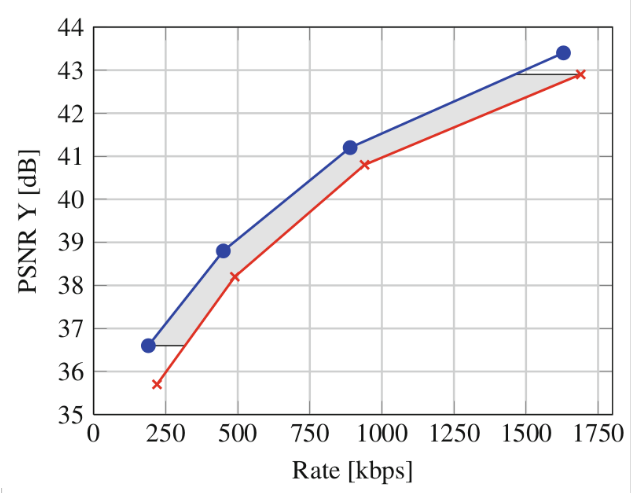
\includegraphics[width=0.3\textwidth]{figures/chartbdrate.png}
	\label{fig:chart_barate}
\end{figure}
\FloatBarrier


In~\cite{Mathias}, the BD-Rate is exemplified by means of Figure~\ref{fig:chart_barate}, where the curves are further drawn by linear interpolation. For the BD calculations, the rate axis is logarithmized and the rate-distortion curves are interpolated by an advanced interpolation method. The overlapping portions of the rate-distortion curves are used for calculation of the BD values. Depending on the range of overlap of the two curves, the resulting BD measurements get more or less meaningful. Therefore, a careful interpretation of the resulting numbers is required.


%\begin{equation} 	\centering 	\label{deltar} 	\Delta R = \frac{R_{B}(D) - R_{A}(D)}{R_{A}(D)}		 \end{equation}


\section{Related Works}

In the literature it is possible to find several studies related to HEVC optimization techniques. Usually the methodological characteristics used in the development of the new technique as metrics and videos used are presented, besides the obtained results. However the test stage is vaguely mentioned or simply has its description ignored. As it happens in~\cite{oliveira:16}, an alternative is presented that uses machine learning to predict the partitioning of the macroblocks and to avoid the extra processing, and the proposed solution is compared with the HM reference encoder. In~\cite{Wang:16}, a parallel approach is used to accelerate coding by distributing multi-core processor efforts. And in~\cite{wang:13}, it is proposed an optimized partitioning algorithm, which refer to a scenario where the coded videos are processed by metrics and then the results are compared, without the aid of a tool for extraction and calculation.

The alternative proposed in~\cite{msu:16} offers an encoder comparison service, in which several configurations are predefined for the tests. For this, it is necessary to submit the encoder to one of the paid or free services offered. Considering the best service, the premium, includes the SSIM, PSNR objective metrics and subjective metrics psycho visual enhancements, also includes the configurations High Speed, Normal and High. Quality, and presets analysis of systhetic motion, distortion in tail area and spatially variable noise. However, this alternative requires payment for more complex tests and also limits testing to a fixed number of configurations and test cases. In addition, more current and advanced metrics like BD-Rate and BD-PSNR are not mentioned. The postponed solution also uses as reference encoders implemented based on X.265, for UHD video tests, this encoder is constantly mentioned in the literature, however the test scenarios proposed by the JVET specify HM encoders. These specifications help to standardize and document studies on the enhancement of the HEVC encoder. The free service offers tests similar to the paid one, but with the reduced number of videos, metrics and reports.

%colocar aqui um breve parágrafo mostrando o que o seu trabalho oferece de inovador com relação aos descritos


\section{Tool Description}

To verify the efficiency of an encoders it is necessary to perform several tests, in which the encoder under test is executed in several coding scenarios, and then the results for each scenario are compared with the results obtained using the reference encoder. Each test sequence of an encoder can last for hours, depending on the videos and test settings, which hinders the development stage. The comparison is made based on values such as bit rate, PSNR, coding time, and so on. These values are generated automatically by the HM encoder and are saved in log files. However, for their use it is necessary to manually collect in each log file, which is a repetitive work and can result in errors from human failure. 

The tool developed in this work executes instances of the modified encoder and reference encoder in all required configurations and then automatically collects all the information necessary for the comparison. With the data collected from the log files the calculation of the Bjontegaard \cite{Bjontegaard} metric is performed. HM-based encoders offer a decoded output video, these videos are used by objective metrics SSIM, PW-SSIM, and so on. to calculate the image quality after encoding. The tool architecture is shown in Figure \ref{fig:fluxo}. 

%colocar as outras métricas


%%usar a mesma fonte do texto
\FloatBarrier
\begin{figure}[!ht]
	\centering
	\caption{Tool architecture.}
	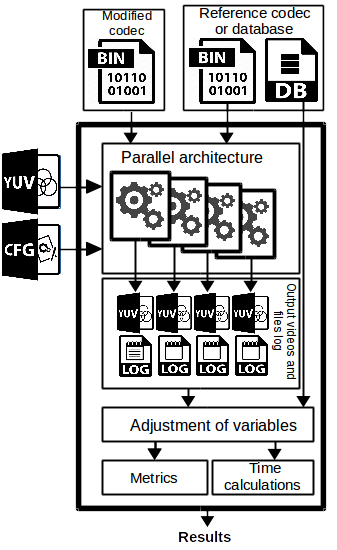
\includegraphics[width=0.47\textwidth]{figures/fluxo.png}
	\label{fig:fluxo}	
\end{figure}
\FloatBarrier

The modular architecture of the tool enables other metrics to make use of the encoding values. To reduce the time of the tests, the tool was implemented in a parallel architecture in which multiple instances of the encoder are executed simultaneously, thus considerably reducing the time of a test. For this, is necessary a adequate management is required so that the execution of different threads does not compromise the integrity of the values used to calculate the metrics, time and other information present in the sequence of tests.

To prevent data loss during an unexpectedly stopped execution, a tool log file is generated that saves the current state of the test and makes it possible to return from where it left off. It is also possible to save the data of the tests performed by the encoders, thus avoiding to repeat the process and thus to promote the construction of a database with the results of the tests.

To execute the tests, the tool receives the parameters specified in Table \ref{parameter_tool}, these parameters indicate the settings that will be addressed equally by the modified encoder and the reference encoder that will generate different outputs. If the parameters are not informed, default values will be used that will execute the tool using a CIF video (352x288) and a one of the standard settings (Random Access Encoding). These parameters have minimum specifications only for checking the operation of the tool. It is important to check the memory and thread limitations before running the tool, it is recommended to run one thread for every two GBs of RAM. In case of an unexpected interruption, the execution of the tool with the -bkp flag activates the backup and the test will return to the moment of interruption.

\FloatBarrier

\begin{table}[!ht]

\centering
\caption{Parameters for tool execution.}
\label{parameter_tool}
\renewcommand*{\arraystretch}{1.5}
\small
\begin{tabular}{|l|l|p{4cm}|l|}
\hline
\textbf{Command} & \textbf{Example}      & \textbf{Description}                                         \\ \hline
./CodecTest      & --                    & Tool executable                                                             \\ \hline
-thr             & 2                     & Number of threads                                            \\ \hline
-vin             & 1 path/video.yuv  & Number of video followed by the video files                  \\ \hline
-cfg             & 1 path/File.cfg & Number of configuration followed by the configurations files \\ \hline
-outl            & path/out/logs/      & Path where log files will go                                 \\ \hline
-outv            & path/outvideos/    & Path where encoded videos will go                            \\ \hline
-eva             & path/BinEncoder    & Rated encoder binary                                         \\ \hline
-ref             & path/BinEncoder    & Reference encoder binary                                     \\ \hline
-fr              & 30                    & Frame rate                                                   \\ \hline
-f               & 130                   & Number of frames                                             \\ \hline
-q             	 & 4 22 27 32 37        & Number of quantization followed by the quantization values   \\ 
\hline
-wdt             & 3840                  & Video width                                                  \\ \hline
-hgt             & 2160                  & Video height                                                 \\ \hline
-bkp             & --                    & Backup flag                                                  \\ \hline
\end{tabular}
\end{table}
\FloatBarrier

To calculate metrics such as PSNR, SSIM among others, it is necessary to execute at least one coding with the modified coder and one of the reference coder, using the same configuration and the same input video, and finally calculate the metrics on the resulting videos . In the case of the metric proposed by Bjontegaard, four executions are required for each encoder, one execution for each QP, totaling eight executions. A execution of a simple test case, in which there are eight executions, for each pair of encoder videos with the corresponding QP, the conventional metrics are calculated, and at the end of the eight executions the Bjontegaard metric is calculated. The tool also enables more extensive test case where you can increase the number of QP, number of videos or settings. The output file structure of the testing tool presents the key information about the execution of each instance, in addition to the total time values and the values of the metrics. A log file example is shown in Figure~\ref{fig:log}.

\FloatBarrier

\begin{figure}[!ht]
	\centering
	\caption{File log example.}
	\fbox{
	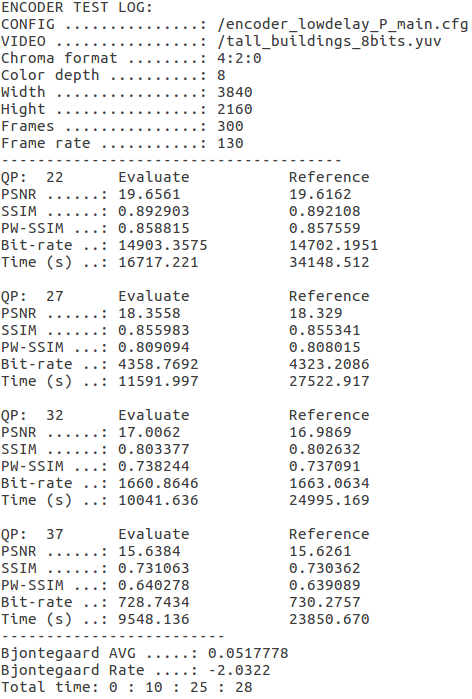
\includegraphics[width=0.45\textwidth]{figures/log.png}
	}
	\label{fig:log}
\end{figure}

\FloatBarrier

This type of visualization helps developers to identify the main differences in the final result between their respective encoders and the original version.

It is also possible to observe the values of Bit Rate per QP used in the test in the Figure~\ref{bitrate_qp}, and also the PSNR values by Bit rate in the Figure~\ref{psnr_qp}, in Figures~\ref{psnr_bitrate} and~\ref{ssim_qp},~\ref{pwssim_qp} there are other ways of displaying the results, in the Figure~\ref{time_qp} present the graph of the time variation between the videos encoded by each QP. These graphs are generated automatically after the tool execution, for this, was used the Gnuplot and LibBoost libraries.

\FloatBarrier
\begin{figure}[!htb]
	\centering
	\caption{Bit Rate x QP.}
	\fbox{
		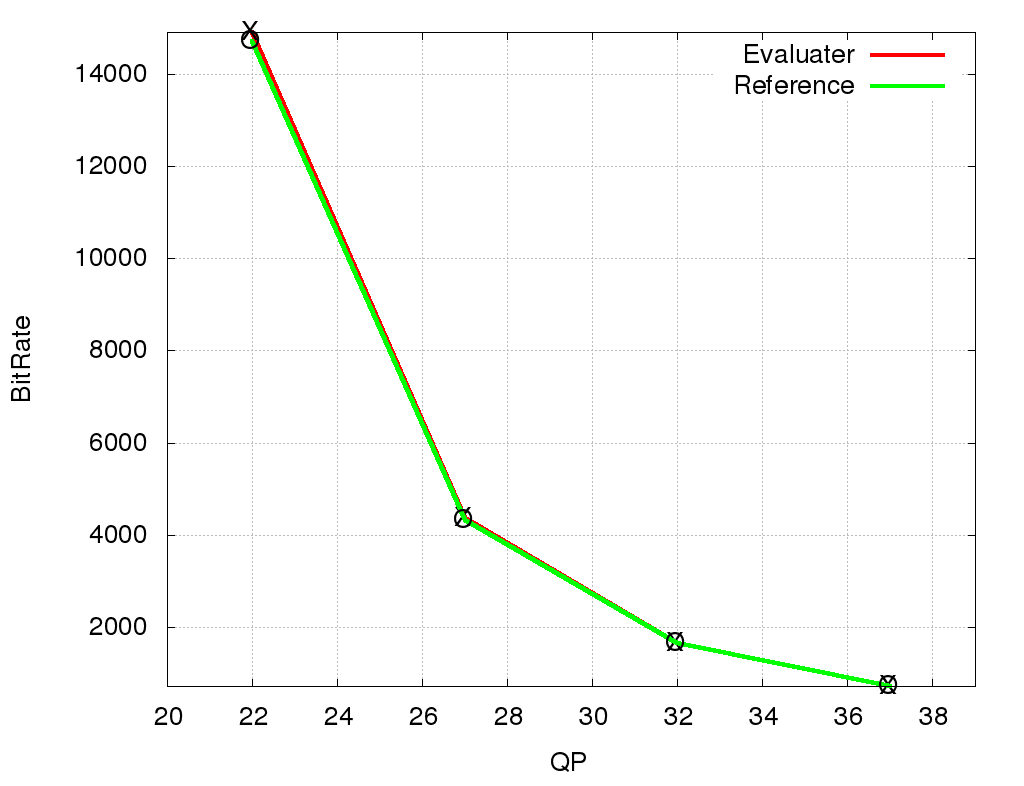
\includegraphics[width=6cm]{figures/bitrate_qp.png}
		\label{bitrate_qp}
	}
	\end{figure}

\begin{figure}[!htb]
	\centering
	\caption{PSNR x QP.}
	\fbox{
		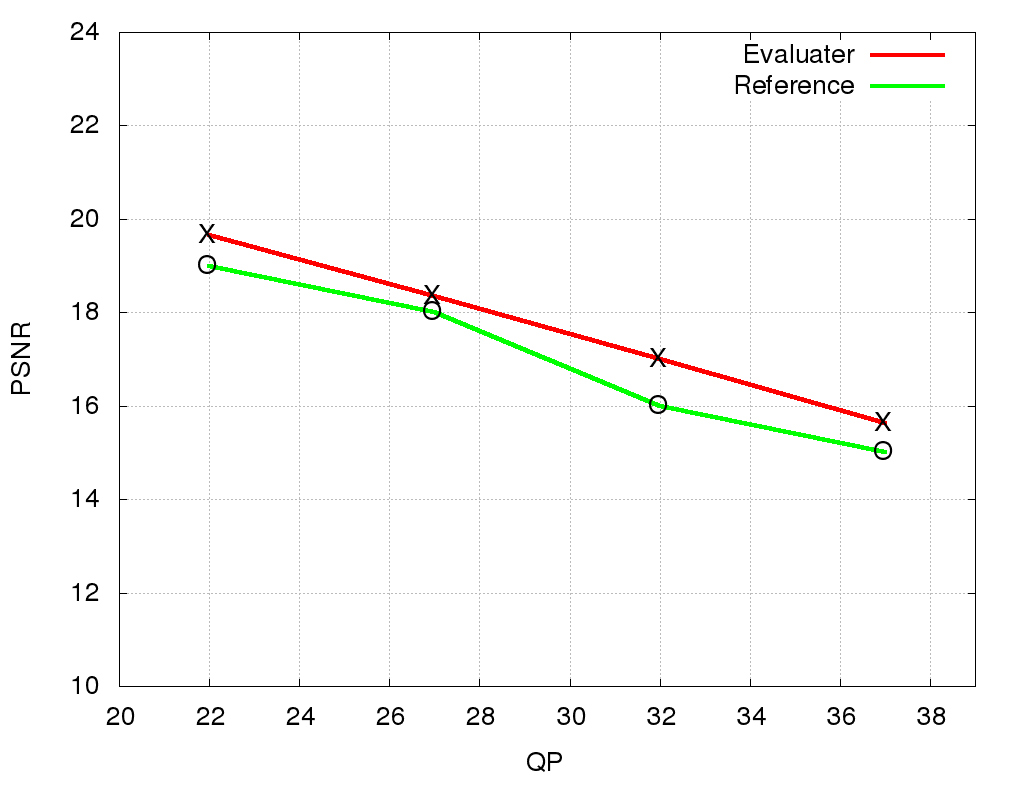
\includegraphics[width=6cm]{figures/psnr_qp.png}
		\label{psnr_qp}
	}
\end{figure}


\begin{figure}[!htb]
	\centering
	\caption{PSNR x BitRate.}
	\fbox{
		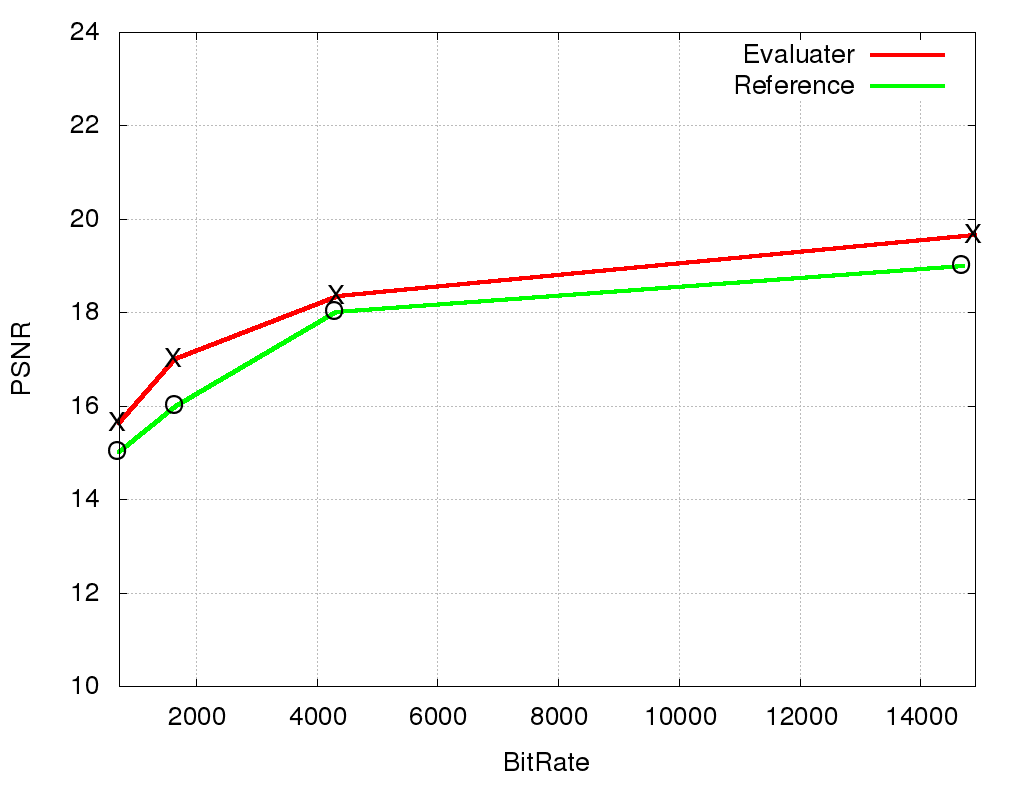
\includegraphics[width=6cm]{figures/psnr_bitrate.png}
		\label{psnr_bitrate}
	}	
\end{figure}
\begin{figure}[!htb]
	\centering
	\caption{SSIM x QP.}
	\fbox{
		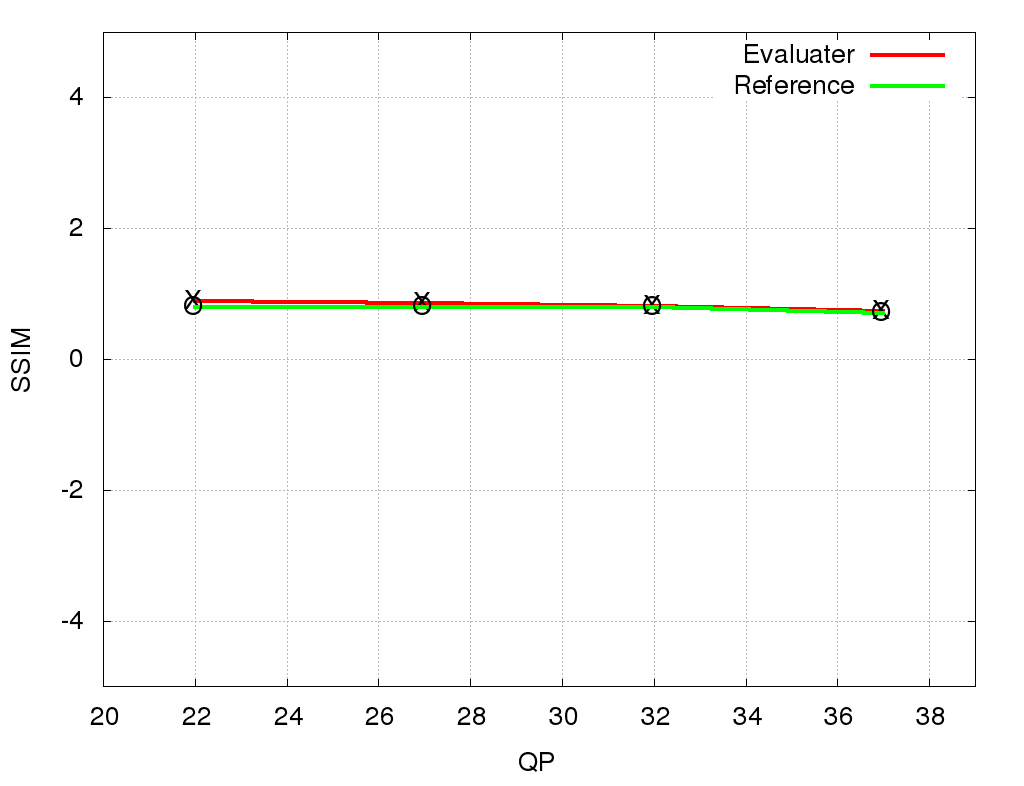
\includegraphics[width=6cm]{figures/ssim_qp.png}
		\label{ssim_qp}
	}
\end{figure}	
\begin{figure}[!htb]
	\centering
	\caption{PWSSIM x QP.}
	\fbox{
		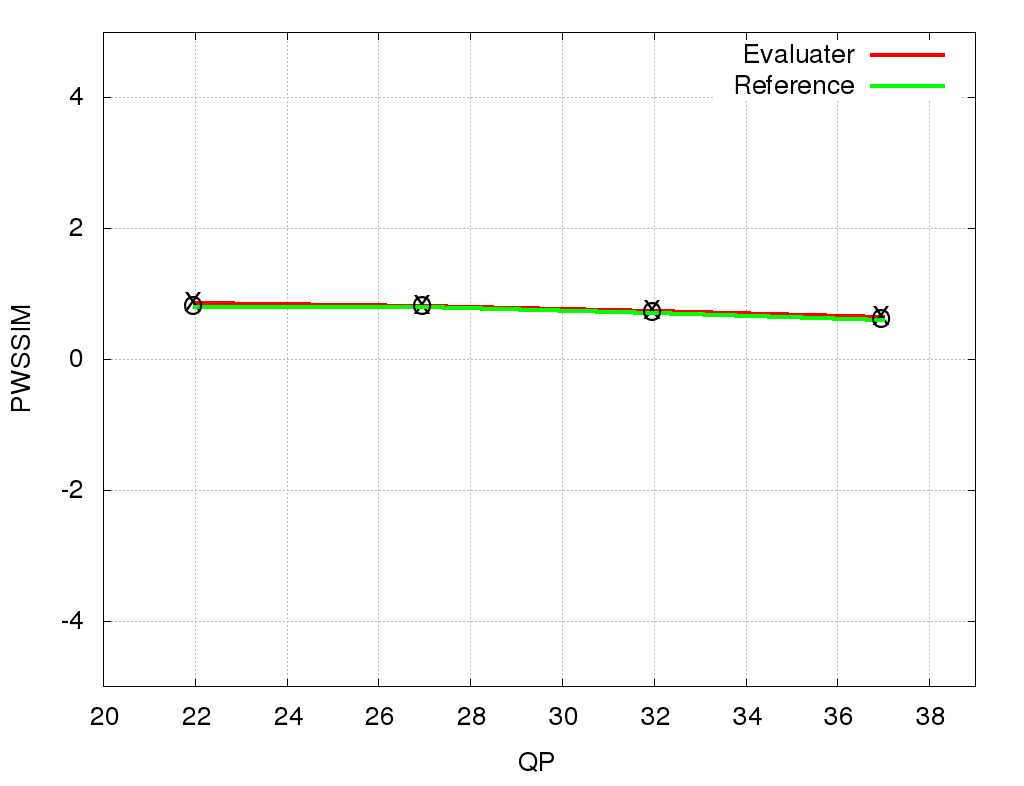
\includegraphics[width=6cm]{figures/pwssim_qp.png}
		\label{pwssim_qp}
	}
\end{figure}	
\begin{figure}[!htb]
	\centering
	\caption{Time x QP.}
	\fbox{
		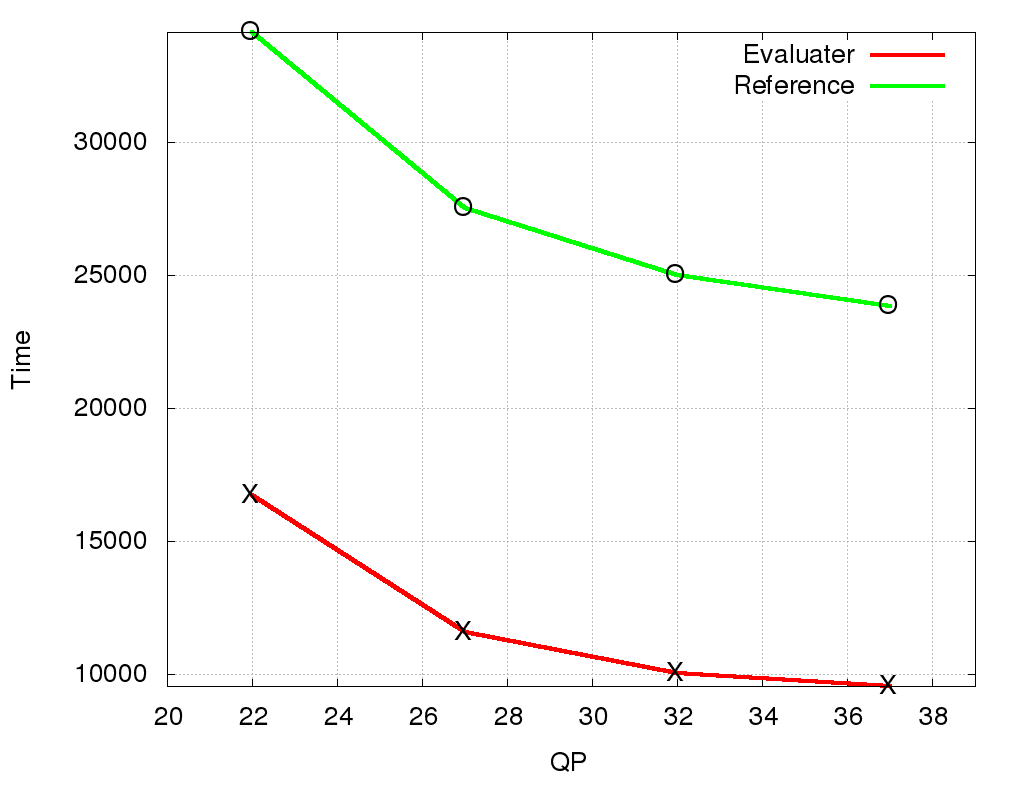
\includegraphics[width=6cm]{figures/time_qp.png}
		\label{time_qp}
	}
\end{figure}
\FloatBarrier

%\pagebreak

\section{Result}

To validate the tool, the modified version of the HM.16 encoder proposed in \cite{oliveira:16} was evaluated, using the original version of the encoder as reference. The test was performed on a computer with AMD FX-8320 processor (8 cores), 32 GBs of RAM and Ubuntu 16.04 operating system. The 4K sequences used are available in \cite{sjtu:17}, this videos has a frame rate of 30 fps, and 8 bits per color component, in a total of 600 frames.

During the tests, the tool showed a mean time reduction was approximately 81,2\%. In a simple test case, for example, the total time spent executing the encoders and calculating the metrics using multi-threaded processing was 8  hours while the same test performed in a conventional scenario, ie running one instance of the encoder at a time, running the metrics independently and collecting data from the log files, was 1 day, 19 hours and 28 minutes, without considering the time for data collection in the log files. In Table \ref{tests_configs}, presents the results in the time reduction percentage in other test cases, using the configurations presented in Section \ref{config} and videos available in \cite{sjtu:17}.


\FloatBarrier
\begin{table}[!ht]
\centering
\caption{Tests results.}
\label{tests_configs}
\renewcommand*{\arraystretch}{1.5}
\small

\begin{tabular}{|l|l|l|l|}
\hline
\textbf{Config}				& \textbf{Video} 		&		\textbf{Time reduction}		\\ \hline
All Intra					& Library				&		81,2\%						\\ \hline
Low Delay B					& Library				&		80,54\%						\\ \hline
Low Delay P					& Library				&		81,81\%						\\ \hline
Low Delay P					& Tall Buildings		&		78,77\%						\\ \hline
Random Access				& Campifire Party		&		81,23\%						\\ \hline
Random Access				& Construction Field	&		79,41\%						\\ \hline

\end{tabular}
\end{table}
\FloatBarrier



\section{Conclusion}

In this work, a tool for automated testing was developed, which aims to assist in the testing stage in the process of developing encoders. For more complex tests, a implementation of a distributed version of the tool is in progress, which will allow the execution of more instances of the encoder according to the configuration and quantity available machines. Online services are also being developed, in which researchers and developers can submit the executable program of their encoders and select the configurations so that the tests are performed on a robust server. With this proposal also intends to build a database fed with the data of the tests of the users, this database will contribute to other researchers.

\bibliographystyle{waslon}
\bibliography{sample}

% that's all folks
\end{document}


